\section{Pooling end-to-end: congestion management}
\label{sec:resourcepooling:congestion}

Much of the value of the Internet is derived from the ability to pool capacity end-to-end: the statistical multiplexing afforded by packet switching resulted in a more efficient network, far better suited to the bursty nature of computer traffic than prevalent circuit switched alternatives. 
Where demand outstrips supply however, congestion arises. 
This is the inevitable consequence of sharing scarce resources, and as such should not be viewed as a problem in and of itself. 
The difficulty lies in resolving this contention both efficiently and fairly. 

\subsection{Historical precursors}

%Baran, 1964, reliability in network, foreshadowing of inevitable.
Early work in defining congestion, and forever ingraining the term in networking nomenclature, can be traced to work on queuing systems by Kleinrock \cite{Kleinrock:1975} beginning from 1961. 
However, it is in the work of Paul Baran at \acs{RAND} \cite{Baran:1964p451} that a deeper concern for the implications of congestion can be found. 

Baran's work on a ``distributed network concept'' \footnote{The term packet switching was yet to be adopted. It would later be imported from similar work by Donald Davies and others at \ac{NPL}.} was intended for military purposes, and as such was required to deal with traffic overload gracefully.
Traffic was expected to be marked by users according to a military precedence system. During times of traffic overload, Baran envisioned a priority control console, operated directly by a military officer, which would regulate the allocation of capacity to each traffic class.
Control was in the network. In part, this reflected military chain of command, but Baran had uncovered an additional cause for concern which would later resurface in the Internet: during times of crisis, users could not be trusted to mark their own traffic:

% users can't be trusted
\begin{quote}
\textit{
Messages once labelled ``Deferred" will be stamped ``Operational Immediate,'' and jammed back into the input hopper. It is analogous to the inflationary competition of competing buyers for scarce goods. We temporarily delude ourselves into thinking that we are buying more capability by inflating the precedence indicator.
}
\end{quote}

Long before such notions would become widespread, Baran had both identified an economic context to congestion and the inherent flaws in precedence marking which would later malign the \ac{IP}. Underlined in the document are two further passages:


\begin{quote}
\textit{
    Communications networks are rarely exercised in real-time to simulate extensive communications network damage and overload.
}
\end{quote}
\begin{quote}
\textit{
    A communication network that does not let the user know how long it will be before his message will be delivered to the end addressee may be theoretically oscillatory.
}
\end{quote}

% resource sharing, who cares?
Both would prove prescient as the \ac{ARPANET} took off in 1969. 
The \ac{ARPANET} was at the helm of an ideological battle between packet switching and circuit switching, and much early work would revolve around the search for an architectural identity. 
While commonly identified as the precursor to the Internet, the \ac{ARPANET} was akin to connection oriented networks such as X.25. Messages would be relayed between \acp{IMP} towards hosts, with each \ac{IMP} ensuring reliable, in-order message delivery.

In the midst of debates over layering or the relative merits of connection and connectionless architectures, there was little interest in understanding how network resources should be shared.  
By and large, there was also no need. 
A combination of abundant capacity, slow terminals and inefficient data protocols ensured that contention was a rare occurrence. 
Initially, hosts could only send one outstanding message at a time, resulting in poor performance which would decrease proportionally to the number of hops in a connection.
By 1971, the peak burst rate recorded between hosts was 40kb/sec using parallel connections, approximately 50\% of bottleneck capacity \cite{Cerf:1974p455}.
Even within such systems, loss, however rare, could prove problematic, and its detection was being debated by Postel and others in 1973 \cite{Postel:1973p462,Hathaway:1973p461}.
It was becoming evident that existing flow control was inefficient. Additionally, end-to-end acknowledgements would be necessary, as Baran had predicted almost a decade in advance.
The death knell for the connection-oriented architecture would come from France, where the CYCLADES \cite{Pouzin:1973p551} network had demonstrated the feasibility of building reliable communications on top of unreliable network elements. 
The simplicity and elegance of this \textit{datagram} network and associated windowed flow control were quickly adopted within \ac{ARPANET}.

% 1974, Cerf/Kahn, TCP, still lots of uncertainty over reliability. 
% Assessment of ARPANET: retransmission and reassembly moved to HOST, 
The specification of the \ac{TCP} \cite{Cerf:2005p452} in 1974 pushed connection establishment, sequencing, flow control and message reassembly towards the end-host.
The architectural blueprint for what would become known as the Internet was almost complete, but not without some loose ends. 
For one, the \textit{Internetwork header} conflated seemingly different functions. 
By 1975, efforts had begun to separate the \ac{IP} header from the \ac{TCP} header \footnote{Vestigial traces of this late separation are still evident - to this day the calculation of the \ac{TCP} checksum takes into account the \ac{IP} header.}.
Likewise, the nature of congestion was still not thoroughly understood.
When referring to \ac{TCP} retransmissions, Cerf and Kahn point out that ``the HOST level retransmission mechanism (...) will not be called upon very often in practice. Evidence already exists that individual networks can be effectively constructed without this feature''. 
In an assessment of \ac{ARPANET} protocols from the same year \cite{Cerf:1974p455}, Cerf lists under unresolved problems and issues that ``the \ac{IMP} subnet must have a way of combating congestion which may result from too rapid influx of data''.
This mechanism would later materialize as the \ac{ICMP} Source Quench option \cite{Postel:1981p463}, whereby routers could notify senders to reduce their rates. 
Alongside \ac{TCP} flow control, it would prove to be the only means of managing congestion as \ac{NCP} was finally replaced by \ac{TCP}/\ac{IP} on Flag Day, 1982.

That more attention was not paid to managing congestion in the eight years between the initial specification of \ac{TCP} and its eventual deployment is unfortunate. 
However, there was little indication as to the potential gravity of the problem.
By 1982, there were still only 235 hosts on the Internet \cite{Lottor:1992p459}. 
Most of these would have been attached to packet switches over protocols providing flow control such as X.25. 
Furthermore, there were more pressing concerns elsewhere. Work was under way in refining applications which would drive initial demand. Addressing and routing posed scalability concerns as it became clear that the number of potential networks would rapidly exceed the limit of 256 seen as sufficient only a few years earlier \cite{Cerf:2005p452}. The host table was becoming too large to distribute as a single file and so distributed alternatives were needed \cite{Mockapetris:1987p527,Birrell:1981p457}. With no progress on any of these it is unlikely the Internet would have become large enough to become a victim of its own success.

Finally, extensively testing how the network would operate under load was never an option. 
Unlike contemporary packet switched networks such as CYCLADES, the \ac{ARPANET} had always been too \textit{useful} to be anything but a production network \cite{Day:2010p187}. 
Within four years of Flag Day the number of hosts would increase tenfold and connectionless \acp{LAN} would become widespread. 
By 1986, congestion collapse was recurrent as hosts persisted in retransmitting packets into an overloaded core.
Baran's vision of a packet-switched network had come full circle.

\subsection{\acs{TCP} congestion control}
\label{sec:resourcepooling:tcp}

%Nagle, etc
The importance of congestion control within \ac{TCP} was first highlighted by Nagle \cite{Nagle:1984p458} in 1984. 
Working at Ford Motor Company, which operated the only private \ac{TCP}/\ac{IP} long-haul network at the time, Nagle reported periods of excessive load and unusual congestion problems. 
Nagle proposed alterations to address the small-packet problem, in which an excessive number of small packets were generated for the transmission of keyboard strokes, and to improve the handling of \ac{ICMP} Source Quench messages. 
Neither would prove sufficient in the long run.  
As issues arising from congestion increased, so too did the interest within the community to address the problem. 
Independent work by Jain and Ramakrishnan at \ac{DEC}, Phil Karn, Lixia Zhang and Craig Partridge had all begun to converge on similar solutions for managing congestion, but ultimately it would be Van Jacobson who would synthesize the model for congestion control which is still prevalent today.

%VJ
% packet conservation principle
In \cite{Jacobson:1988p398}, Van Jacobson begins by asserting that for a system to be stable each connection should abide by a ``packet conservation principle'': a new packet should not enter the system until an old packet leaves \footnote{While often attributed to Van Jacobson, the concept of packet conservation was not new. Its origins can be traced at least as far back as 1972, when Donald Davies proposed a similar ``isarithmic'' approach for controlling congestion within networks \cite{Davies:1972p473}.}. 
Building on this intuition, two separate moments in a connection lifetime are identified, as shown in figure \ref{fig:tcpcc}. 

Initially, a connection must attempt to reach equilibrium by ramping up its window size during a \textit{slow-start} phase. 
From an initial \acfi{cwnd}, a \ac{TCP} connection increases the congestion window by one packet for each \ac{ACK} received, until congestion is detected or the window size surpasses the \acfi{ssthresh}, an initially predefined system variable.
The resulting increase in the congestion window is exponential, and thus expected to exceed available capacity at most by a factor of 2. 
Prior to the introduction of \textit{slow-start}, this overshoot was potentially much higher as hosts would initiate a connection by immediately adjusting to the receiver's advertised window. 

Upon exiting \textit{slow-start}, a flow is deemed close to equilibrium.
The \ac{TCP} sender moves to the \textit{congestion avoidance} phase, where an \ac{AIMD} strategy is used to probe for available bandwidth. 
In the absence of congestion, the window is increased by one \ac{MSS} every round trip time.
If congestion is detected, the window is halved and \ac{ssthresh} is readjusted to this value.

To signal congestion Van Jacobson settled on packet loss. 
While loss could arise from data corruption, such cases were considered sufficiently rare as not to hinder efficiency. 
Loss provided a poor resolution signal, but was the only form of congestive feedback shared by all networks 
\footnote{\ac{ICMP} source quench, despite being widely deployed, was not a viable solution for reasons described in section \ref{sec:resourcepooling:xcc}.}.
The efficiency of retransmission was further improved by providing a more accurate estimate of the \ac{RTT}, and including a mechanism for \textit{fast retransmit}. 
The resulting changes were quickly deployed as \ac{TCP} Tahoe and proved instrumental in curbing congestion. 


\begin{figure}
    \centering
    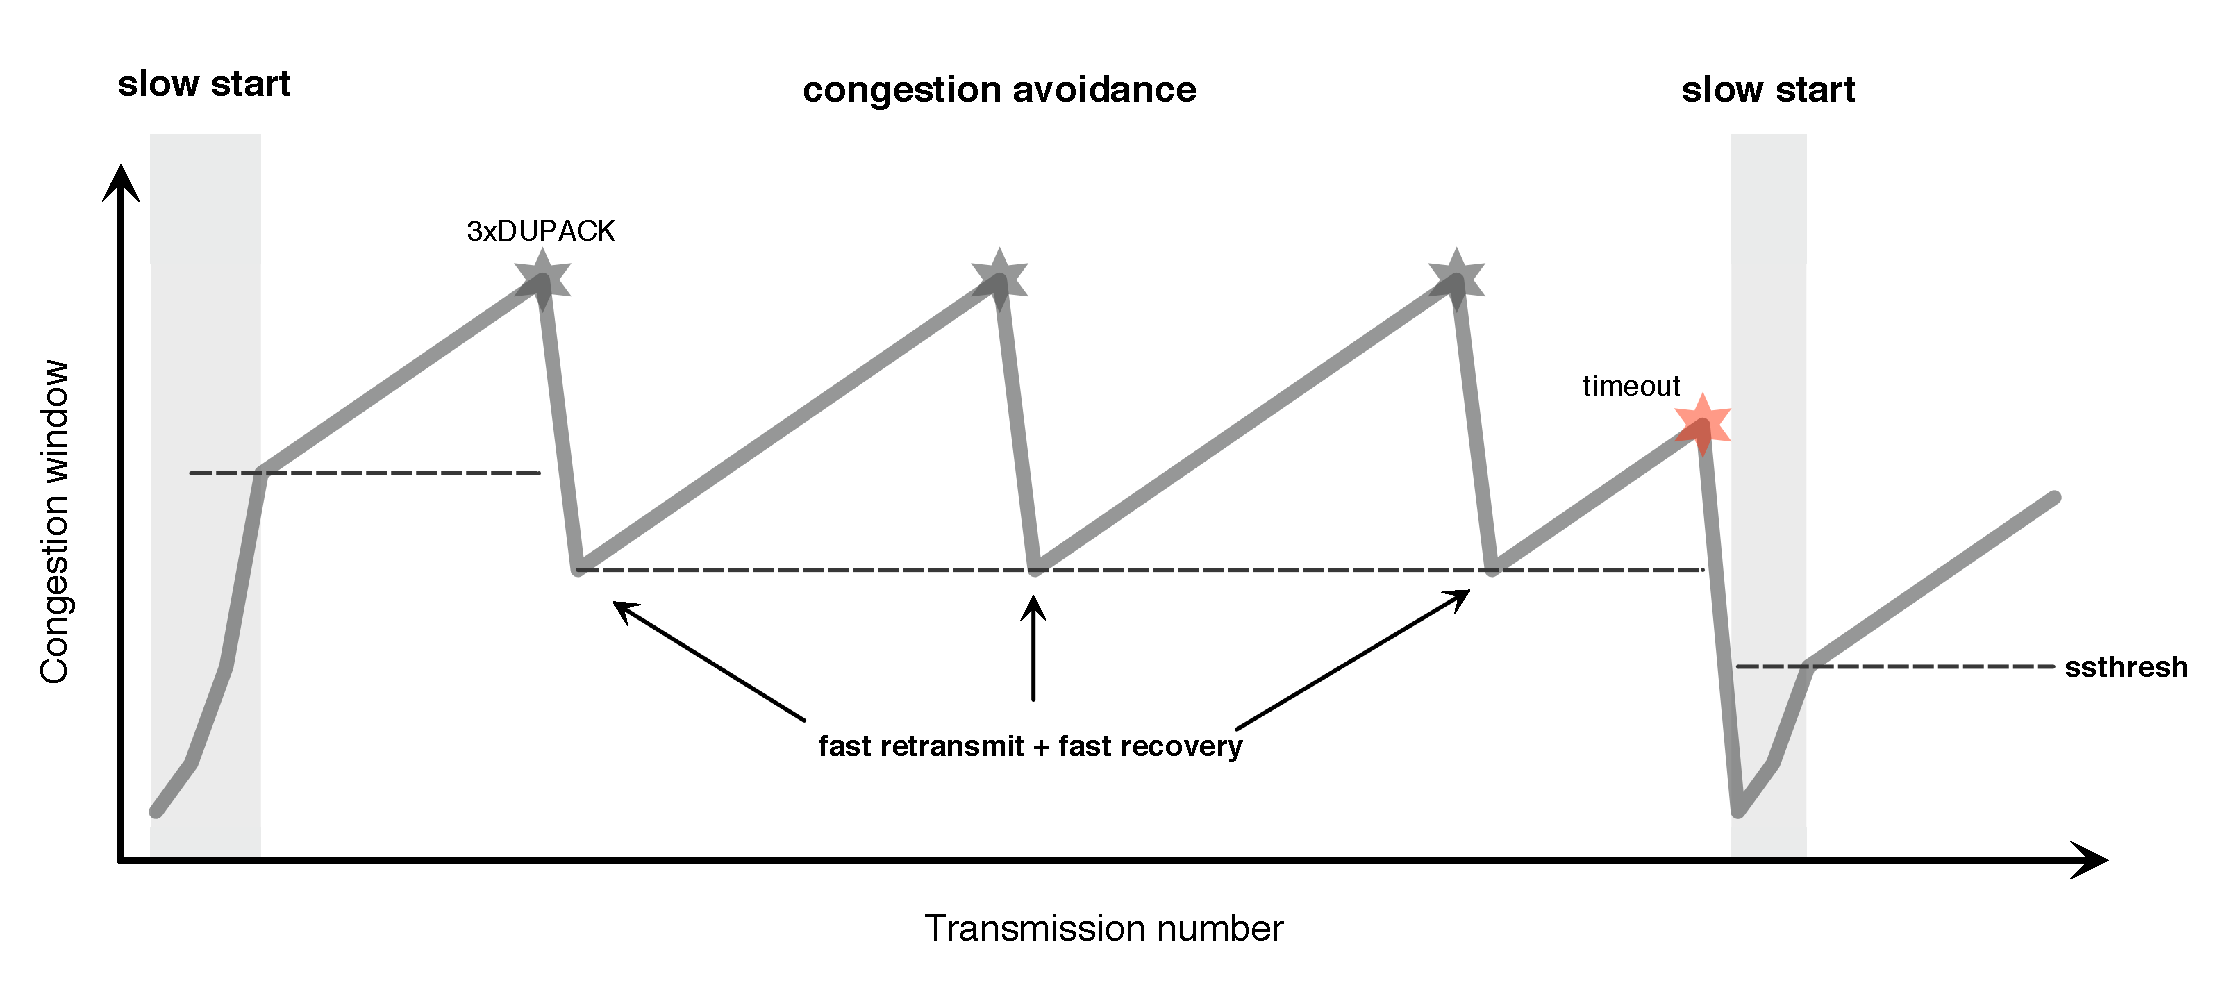
\includegraphics[width=5.0in]{figures/resourcepooling/tcpnewreno}
    \caption{\acs{TCP} congestion control}
    \label{fig:tcpcc}
\end{figure}

Congestion control would go on to become a staple of networking research. Successive refinements, including the addition of \textit{fast recovery} resulted in \ac{TCP} Reno \cite{Stevens:1997p466} and then \ac{TCP} NewReno \cite{Paxson:1999p467}, which would become the most commonly accepted and widely deployed congestion control algorithm for over a decade. Variants such as Vegas \cite{Brakmo:1994p468} and \ac{FAST} \cite{Wei:2006p469} would complement the use of loss with the estimation of queuing delay, and adjust rates accordingly. \ac{BIC} and CUBIC \cite{Xu:2004p470,Ha:2008p471} addressed rate adjustment as a binary search problem and would be adopted by Linux distributions. Finally, \ac{CTCP} \cite{Tan06acompound}, deployed from Windows Vista onwards, would use loss and delay as a combined congestion signal, tracking both as separate components before calculating an overall congestion window.

In spite of these changes, the core of \ac{TCP} congestion control algorithms can still be directly traced to Van Jacobson's initial proposal. 
That a stop-gap solution has managed to sustain the growth of the Internet for over two decades is an outcome even Van Jacobson could not have anticipated. 
In \cite{Jacobson:1988p398}, concern is expressed in that ``the congestion control noise sensitivity is quadratic in $w$ but it will take at least another generation of network evolution to reach window sizes where this will be significant''. 
Despite work to address such inherent scaling issues \cite{Mathis:2009p309,Kelly:2003p475}, \ac{TCP} has remained unchanged - as bandwidth increases so too will the time between loss events.
Likewise, while \ac{TCP} shares bandwidth efficiently, there was no claim the outcome would be fair. In describing future work, Van Jacobson observes that ``only in gateways, at the convergence of flows, is there enough information to control sharing and fair allocation''. 
Over the coming years, congestion management would slowly seep into the network.

%In the aftermath of TCP Tahoe, Van Jacobson and others would investigate AQM techniques to manage buffer occupancy \cite{}. 
%More broadly, the most significant changes to congestion management over the next decades would result from a shift in control from the hosts into the network.

%missing topics: flow fairness, scale 1/p


\subsection{Traffic shaping}
\label{sec:resourcepooling:shaping}

% why it matters
The introduction of congestion control in \ac{TCP} addressed the growing pains as the Internet scaled to become a network of networks.
Congestion however plays an equally important role within networks.
On a short time scale, there is a variable cost which an operator must pay its own providers for transit traffic. 
On a longer time scale, there is a fixed cost in upgrading capacity at each provisioning cycle.
By minimizing congestion, operators hope to reduce both. 

% provider definition of congestion, pricing.
From a provider's perspective, congestion is commonly defined as the average utilization of a link over some period of time. 
Under this definition, the most congested link does not necessarily experience the highest packet loss, but rather exhibits the highest utilization over an extended period of time.
This reflects the volume-based pricing models typically used between networks, the most common of which is 95th percentile pricing.
Under such a scheme, aggregate traffic rates are calculated over each time window of duration $t$.
At the end of each billing cycle, time windows are ordered by traffic rate, of which the highest 5\% are discarded.
The largest remaining traffic rate represents the 95th percentile rate that is used to charge customers.
Inbound and outbound traffic are usually tracked separately, of which only the most significant is charged.

Both hosts and network remain intent in reducing their own view of congestion, but in doing so pursue potentially disparate objective functions.
Over time, the changing nature of Internet traffic, technology and stakeholders has exacerbated this tussle \cite{Clark:2005p67}.
In \cite{Bauer:2009p200}, Bauer et al.\ characterize the evolution of Internet traffic into three phases:

\begin{itemize}
    \item{Prior to the 1990s, the Internet was largely confined to academic and research purposes. 
        Congestion typically occurred within the core, as long haul lines would often trail behind local area networks in terms of bandwidth. 
        Traffic was dominated by a small number of applications - mail, bulk file transfer and low bandwidth interactive sessions - all of which were tolerant of congestion.
        Furthermore, the Internet was still small enough that congestion was viewed as a shared concern to be jointly addressed by the community.
    }
    \item{By the 1990s the commercialization of the Internet was in full swing, attaining mass market status as residential users signed up for dial-up access.
    The dramatic increase in user base was somewhat attenuated by the existence of a bottleneck at the edge.
    Dial-up offered low data rates of up to 56.6kb/s and intermittent connectivity, both of which were instrumental in curbing demand.
    The most significant new application protocol, \ac{HTTP}, put more demands on end systems than on the network, as web servers scaled to cope with thousands of simultaneous requests.
    Congestion within the network was rare and most likely to occur at data modem banks which would in effect perform admission control - excess subscribers attempting to connect would receive a busy signal.
    }
    \item{Since 2000, the advent of broadband access lifted bandwidth constraints at the edge and pushed congestion deeper into \acp{ISP}.
            Higher data rates coupled with ``always on'' connectivity led to a much larger set of applications placing different demands on the network, from bandwidth hungry file sharing to congestion sensitive \ac{VoIP} or video streaming.
    Network provisioning, previously driven by the needs of commercial clients, would become increasingly driven by the usage patterns of residential customers. 
    }
\end{itemize}

The proliferation of media-rich applications led to a growing disparity between customers.
A minority of ``heavy'' users incurred the majority of costs from pooling available bandwidth despite paying the same flat fee as remaining ``light'' users.
In the long term, capacity upgrades would prove ineffective in quenching demand from the former group while passing unwarranted costs onto the latter.
Faced with a deluge of data and having to satisfy the needs of a diverse range of both applications and customers, network operators inevitably took it upon themselves to manage congestion.

The Internet architecture however does not provide the means for a network to manage congestion effectively.
Furthermore, the communal approach to addressing problems had since grown into a cumbersome and convoluted standardization process within the \ac{IETF} \cite{Bush:2005p476}.
Unsurprisingly, operators quickly resorted to piecewise solutions to artificially stifle demand with little consideration on the wider impact of their actions. These attempts at \emph{traffic shaping} would take on a variety of forms.

One method of reducing congestion is by limiting the total volume of traffic a subscriber can send or receive over a given period and applying penalties should this cap be exceeded.
This method imposes the least technical requirements as volume accounting is already widely performed.
While volume capping introduces an expected upper bound for the volume of traffic traversing a network over each billing cycle, it fails to address demand patterns over shorter time scales.
Subscribers within their volume allowance can still cause considerable congestion by acting synchronously, for example by being active during peak hours only. 
Conversely, volume capping unnecessarily penalizes applications which shift their traffic towards less congested periods. 

Alternatively, congestion can be potentially reduced by throttling throughput. 
By imposing rate limits during periods of oversubscription, providers may attenuate the impact any single traffic source can have on others.
Doing so efficiently however is challenging.
For one, available capacity and periods of congestion cannot easily be narrowed to a single throughput threshold or time period.
In provisioning rates for the worst expected case, providers forsake efficiency when contention may not arise.
Furthermore, throttling can be performed on a per-customer or per-flow basis.
In the former case, throttling fails to take into account how much shared capacity a customer has occupied over time, degrading performance equally for heavy and light users alike.
Throttling flows on the other hand may prioritize types of traffic for applications using specific port ranges. 
Applications affected by such network policing will however tend to adapt over time, either by changing port or increasing the number of flows to bypass throttling.

Volume capping and rate throttling are necessarily naive and inefficient as they can function on network layer information alone, but in doing so are largely benign.
Either method however can be performed selectively by inspecting packet contents in order to prioritize traffic.
These attempts at \ac{DPI} have had a much more nefarious effect on the Internet.
The introduction of \ac{DPI} middleboxes break layering, introduce complexity within the network and hinder the deployment of new, innovative applications and transport protocols at the edge.
Applications targeted by \ac{DPI} have become increasingly stealthy, often masquerading as \ac{HTTP} traffic.
The ensuing arms race between traffic obfuscation and traffic identification methods has been waged at great cost to the Internet as a whole and little benefit to any stakeholder in particular.

In addressing the tussle surrounding congestion, transport and network communities applied successive independent fixes rather than reaching a compromise within a common architectural solution.
Over time, the damage caused in adopting the former has only strengthened the arguments for the latter.

\subsection{Explicit congestion control}
\label{sec:resourcepooling:xcc}

In previous sections unilateral solutions to congestion management were reviewed, where either end-hosts or networks perform their duties in isolation. 
The overbearing dominance of the transport layer in resource sharing was shown to be an ex post construct:
neither Baran \cite{Baran:1964p453}, Cerf \cite{Cerf:2005p452} or, for that matter, Van Jacobson \cite{Jacobson:1988p398} envisaged an Internet where control was exerted from the edges alone.
This section reviews proposals where both endpoints and network share responsibility for managing congestion through the use of explicit congestion control, whereby sources adjust sending rates according to explicit network feedback.

% source quench
There have been enough failed attempts at deploying explicit congestion control on the Internet that it has become common to overlook the fact it was once the dominant model for congestion management.
Prior to \ac{TCP} congestion control, hosts performed end-to-end flow control alone. 
While most underlying data layer protocols provided some degree of flow control, gateways could signal overload by sending \ac{ICMP} source quench messages to sources.
Hosts were then expected to reduce sending rates upon receiving this explicit feedback from the network.
Unfortunately, the source quench mechanism was marred with oversights.
The specification of \acs{ICMP}\cite{Postel:1981p463} stated that source quench messages ``may'' be sent by gateways for every packet it discards.
However it also allowed source quench messages to be emitted by gateways approaching, rather than exceeding, their capacity limit.
As a result, upon being cautioned by a gateway a sender had no indication of whether the packet at fault had been discarded.
Under such circumstances, the source host ``should cut back the rate (...) until it no longer receives source quench messages from the gateway'',
but no further indication on how such a goal can be attained was provided.
Confusingly, destination hosts could also emit source quench messages if overcome by processing, duplicating functionality already present at the transport layer \cite{Postel:1980p445}.

Source quench was inevitably deprecated \cite{Baker:1995p479}, crippled by overloaded semantics and a lack of obligation or guidance for sender compliance.
In retrospect, source quench messages represented an attempt at doing \emph{too little, too early} \cite{Crowcroft:2003p450}.
Endpoint congestion control would only come of age with \ac{TCP} Tahoe.
Prior to the continuous control theory mechanisms introduced by Van Jacobson, Jain, and others, there was no framework within which explicit feedback could be modelled.
Only with the onset of congestion collapse events did many of the frailties of source quench messages become apparent.
There was no understanding of the problem at hand until it was too late.

%DECbit
Despite this failed first attempt, interest in applying explicit network feedback to the Internet did not wane.
In 1988 Jain and Ramakrishnan proposed an explicit binary feedback scheme for congestion avoidance which would evolve into DECbit \cite{Ramakrishnan:1990p456}.
Under such a scheme, the network header would contain a single bit which could be toggled by intermediate routers experiencing the onset of congestion.
The resulting bit would then be returned to the sender.
If at least half of the previous congestion window had been marked, the sender would decrease its window by 7/8, otherwise it would continue to increase its sending rate additively.

%ECN
DECbit proved promising enough to be ported to \ac{IP} with minor changes as the \ac{ECN} protocol \cite{Floyd:1994p491}.
\ac{ECN} would reuse two bits from the \ac{ToS} field to retrieve binary network feedback.
If neither bit was set, a packet is deemed to be non-\ac{ECT} and therefore legacy traffic.
If either bit was set, both hosts had established the usage of \ac{ECN} during the initial handshake and the packet belongs to an \ac{ECT} flow.
Having detected the onset of congestion according to a given \ac{AQM} discipline, an \ac{ECN} aware queue would then set both bits to encode the \ac{CE} code point.
Unlike DECbit, a single \ac{CE} marking would be sufficient motive for a sender to decrease its congestion window, making \ac{ECN} compatible with probabilistic \ac{AQM} mechanisms such as \ac{RED} \cite{Floyd:1993p492}.
Furthermore, the multiplicative decrease was more conservative than in DECbit, and followed the existing \ac{TCP} standard of halving the congestion window.
This conscious decision to make \ac{ECN} enabled traffic perform similarly to legacy \ac{TCP} over large time scales would strip it of a potentially important competitive advantage in deployment whilst retaining one of the less scalable components of \ac{TCP}.

Both DECbit and \ac{ECN} proved to be \emph{too little, too late}. 
Proposed at the same time as \ac{TCP} congestion control, DECbit was initially shunned in favour of a practical solution which could be rapidly deployed and rectified.
By the time sufficient experience with binary explicit feedback had been gained through deployment in DECnet, the Internet had dramatically changed.
The standardization of \ac{ECN} \cite{Ramakrishnan:2001p45} arrived in an Internet overrun by commercial interests which neither understood the problem nor valued the solution. 
As the Internet scaled in size, so too did its inertia to change, ossifying architecturally around a core set of protocols.
Each new addition would be required to address an otherwise unassailable problem.
In an era of dial-up access and rapid roll-out of improvements in \ac{TCP} congestion control, \ac{ECN} seemed like a costly anachronism.
Deployment was further hampered by broken \ac{TCP} implementations and routers which could adversely affect connection establishment for \ac{ECN} enabled traffic.
Despite improvements \cite{Kuzmanovic:2005p118} \ac{ECN} remains poorly used and turned off by default on hosts and routers alike \cite{Bauer:2011p482}.

Ironically for a protocol which has been plagued by deployment issues, the widespread availability of \ac{ECN} in commodity network equipment may yet reassert its relevance. 
Proposals such as re-\ac{ECN} \cite{Briscoe:2005p346} leverage \ac{ECN} in order to achieve cost fairness.
\ac{VCP} \cite{YongXia:2008p121} overrides \ac{ECN} semantics to provide an additional bit of congestion information per packet.
\ac{DCTCP} \cite{Alizadeh:2010p356} repurposes \ac{ECN} to achieve high throughput with low buffer usage within a data centre environment.
Rather than reacting to each marking as a potential loss event, \ac{DCTCP} sources reduce their window proportionally to the \emph{fraction} of marked packets.
From a sequence of single bits, \ac{DCTCP} derives and acts upon a multi-bit signal.
Both \ac{DCTCP} and \ac{VCP} retrofit multi-bit network feedback, itself the subject of much research.

% ABR
The first concerted attempt at deploying multi-bit network feedback would arise in \ac{ATM} networks.
\ac{ATM} provided a connection-oriented data link layer over which service categories with different \ac{QoS} constraints would coexist.
In addition to addressing precise throughput and delay requirements through the \ac{CBR} and \ac{VBR} services, \ac{ATM} offered an \ac{ABR} service \cite{Bonomi:1995p481}, catering for applications with vague requirements and intended as a cost-effective means of supporting data traffic.
Applications using \ac{ABR} would specify ranges of acceptable rates which the network would then satisfy through the dynamic allocation of available bandwidth amongst virtual circuits.

ATM was primarily driven by telecom operators who embraced the concept of explicit network control of rates. 
Capitalizing on similar work on DECbit, an \ac{EFCI} code point was integrated into the ATM data header to provide binary feedback on congestion along a path.
In parallel however, research progressed on rate-based feedback, where the network would explicitly provide sources with the allowed sending rate.
Since \ac{ATM} used small, fixed size packets, called \emph{cells}, control information was preferentially provided through different payload types.
As a result, \ac{ABR} sources in addition to sending standard data cells would periodically emit a \ac{RM} cell to communicate requirements and retrieve information from intermediate network nodes.
The \ac{RM} cell contained fields for different parameters of interest, such as the \ac{MCR}, \ac{PCR}, \ac{AIR} or \ac{RDF}.
Upon receiving a \ac{RM} cell, \ac{ATM} switches would readjust the cell payload to reflect local conditions if they could not meet the specified requirements.
The information contained within the updated \ac{RM} cell would then be fed back from the destination to the source, which would readjust their rates accordingly.

\ac{ABR} would prove a prolific source of research in explicit network feedback.
As \ac{ATM} waned in popularity however, so too did research efforts within the context of \ac{ABR}.
In its wake, a wide set of proposals for traffic management, including credit-based and rate-based approaches, had been investigated, often concurrently \cite{Jain:1996p484}.
With little consensus and no unifying vision however, the \ac{ABR} rate-based framework would encompass different mechanisms with often overlapping functionalities: \emph{too much, too early}.

%XCP, RCP
Multi-bit network feedback would resurface applied to Internet traffic with the \ac{XCP} \cite{Katabi:2002p256}.
Taking a clean slate approach, Katabi et al.\ revisited congestion control without the constraints imposed by existing network equipment.
The resulting proposal introduces a shim \emph{congestion header} between the \ac{IP} and \ac{TCP} headers carrying estimates of the flow \ac{RTT} and inter-packet time \cite{Katabi:2007p485}.
Additionally, a \emph{delta\_throughput} field contains the allowed increase in throughput, and is set to the maximum value at the source.
As a packet traverses routers, the value of \emph{delta\_throughput} is updated by routers according to local conditions.
The feedback loop is then closed as destinations copy the value of the inbound \emph{delta\_throughput} field into the outbound \emph{reverse\_feedback} field.
Upon receiving network feedback, the source updates its congestion window according to the function:

\begin{equation}
cwnd = max\left (  cwnd + reverse\_feedback \cdot RTT, MSS\right )
\label{eqn:xcpcwnd}
\end{equation}


While functionally similar to the rate-based framework proposed in \ac{ABR}, \ac{XCP} represented a significant step forward in explicit congestion control.
For one, \ac{XCP} bypassed the need for flow state which was assumed in \ac{ATM} networks.
Secondly, \ac{XCP} specified a cohesive mechanism for redistributing bandwidth as opposed to expecting a variety of methods to coexist.
An \ac{EC} periodically calculates the amount of bandwidth $F$ to be distributed over the following control interval $d$ according to:
\begin{equation}
F=\alpha\cdot\left ( C - input\_bw \right ) - \beta\cdot\frac{q}{d}
\label{eqn:ec}
\end{equation}
where $C$ is the link capacity, $input\_bw$ is the inbound throughput and $q$ is the persistent queue length.
Constants $\alpha$ and $\beta$ are set to ensure stability by weighing the amount of spare bandwidth allocated and the rate at which the queue is drained.
The available bandwidth $F$ is then distributed amongst flows by the \ac{FC}, which calculates the $delta\_throughput$ to be applied for each packet:
\begin{equation}
delta\_throughput = \begin{cases}
\frac{F}{N} \cdot \frac{X}{d} & \text{ if } F> 0 \\ 
F \cdot \frac{s}{input\_bw \cdot d} & \text{ if } F\leq 0 
\end{cases}
\end{equation}
where $N$ is the approximate number of flows, calculated as the sum of inter packet time $X$ normalized by control interval $d$.
If the resulting $delta\_throughput$ is smaller than the existing value in the congestion header, the router updates the field accordingly before forwarding the packet.

Using multi-bit feedback \ac{XCP} achieves high efficiency and stability with negligible queuing delay.
In prioritizing queue drainage and system stability however \ac{XCP} presented a natural performance bias towards long flows.
Under high utilization, only a small proportion of bandwidth would be reshuffled resulting in a potentially slow convergence to flow fair rates for short-lived flows.
Recognizing the importance such flows had in overall user experience, Dukkipati et al.\ proposed the \ac{RCP}.
Building on the explicit congestion control framework proposed by \ac{XCP}, \ac{RCP} emulates processor sharing by emphasizing the \ac{AFCT} rather than delay stability \cite{Dukkipati:2005p78}.
Rather than calculating a change to the source \ac{cwnd}, the equivalent \ac{FC} in an \ac{RCP} system calculates the explicit maximum rate $R$ to be set for flows traversing a router at interval $n$:
\begin{equation}
R_n = R_{n-1} + \frac{F}{N}
\end{equation}
where $N$, the approximate number of active flows, is obtained by:
\begin{equation}
N = \frac{C}{R_{n-1}}
\end{equation}

By setting a single rate for all flows within an \ac{RTT} of flow start, \ac{RCP} rapidly redistributes bandwidth, but does so at the expense of queue stability.
\ac{RCP} proved well suited for web traffic where completion time is often of greater importance than jitter.
As with \ac{XCP}, the requirement for both end systems and bottleneck routers to be overhauled would prove too high a barrier for incremental deployment.
To blame the lack of deployment of either solution on hardware requirements alone however would be disingenuous, and ignoring the most valuable lesson of all. 
Both offered a compelling universal solution to a problem now escalating with pluralism: \emph{too much, too late}.
Many of the shortcomings in \ac{TCP} congestion control are inherent to limitations in the amount of information one can infer from loss.
In hindsight, that proposals as disparate as \ac{XCP} and \ac{RCP} had emerged in spite of a wealth of explicit network feedback signalled a growing lack of consensus within the community on how to move beyond Van Jacobson's legacy. 
By 2007, a tongue-in-cheek rebuttal of flow fairness \cite{Briscoe:2007p261} would only widen this rift.
For a growing minority, the absence of an overarching solution to managing congestion was no longer construed as an inability to provide the right answer, but as a symptom of asking the wrong question.

\subsection{Congestion exposure}

Resource sharing has evolved haphazardly to being performed by end-hosts and network alike. 
This apparent duplication of effort and source of potential conflict suggests a rare lack of foresight within the Internet architecture. 
More confounding however is that unlike other architectural mishaps, such as the conflation of locater and identifier within addressing, the absence of progress regarding a solution is rooted in a lack of consensus in identifying the problem.

A clearer understanding of resource sharing was built over time by importing notions from similar work in economics, where contention for scarce goods is well understood. 
The concept of pricing congestible resources was pondered as early as 1995 \cite{MacKieMason:1995p493}. 
The breakthrough in applying shadow pricing to a network would come through the work of Kelly \cite{Kelly:1998p139}, who both proved that social welfare could be maximised if each pair of hosts were charged in accordance to the congestion they cause, and that under such a model self-interested behaviour would lead to a stable network under a small set of assumptions.
Furthermore Kelly showed that such a scheme could be easily realized by charging a receiver according to the number of bytes marked as having experienced congestion through the use of \ac{ECN} which was still undergoing standardization.
Kelly's work proved a radical departure from conventional wisdom. 
By sharing capacity equally amongst flows \ac{TCP} had been hard-wired with a single concept of fairness.
That social welfare was shown to be maximized only when users were forced to weigh demand according to expected cost suggested that flow fairness was sub-optimal.
As ever the notion of charging a user variable costs proved unpopular \cite{Odlyzko:2004p290}, while charging the receiver instead of the sender proved impractical.
Building on Kelly's work, Briscoe would resolve both shortcomings.

In \cite{Briscoe:2005p346}, Briscoe et al.\ introduce the concept of \emph{re-feedback}.
Re-feedback attempts to correct an information asymmetry in forwarding traffic: a provider often knows less about the quality of service it provides than the sender.
Due to this asymmetry, Kelly correctly identified the receiver-end as the only point where the entirety of path congestion could be accounted for by the network.
Information on congestion provided by \ac{ECN} is fed back from the receiver to the sender in the transport header, and is therefore not visible to routers.
Furthermore, the return path my differ from the forwarding path.
By reintroducing this explicit feedback in the next outbound packet however, a sender can provide the network with information on the state of the forwarding path, albeit with one \ac{RTT} of delay.
Applying re-feedback to \ac{ECN} lead to the specification of re-\ac{ECN} \cite{Briscoe:2008p494}. 
In addition to information on congestion upstream, provided by \ac{ECN}, re-\ac{ECN} introduces the congestion over the entire path from the previous \ac{RTT} in the \ac{IP} header.

\begin{figure}
    \centering
    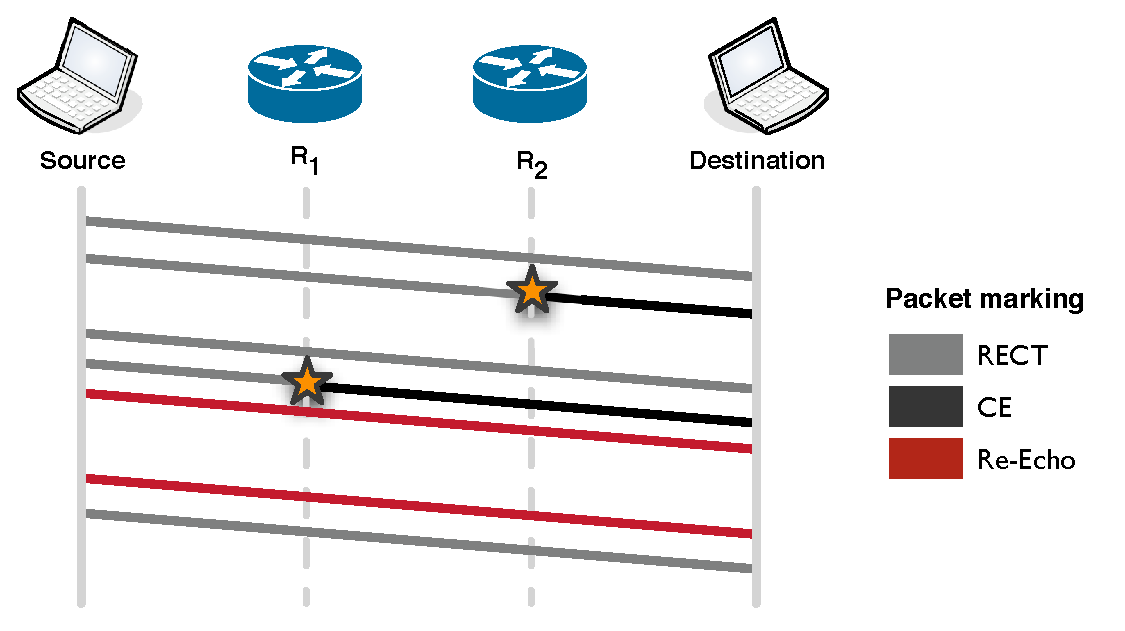
\includegraphics[width=4.0in]{figures/resourcepooling/reecn}
    \caption{Simplified model of re-\acs{ECN}}
    \label{fig:reecn}
\end{figure}

A simplified illustration of how re-\ac{ECN} functions is displayed in figure \ref{fig:reecn}.
A source emits packets with the \ac{RECT} code-point set.
Upon detecting the onset of congestion, a congested resource which is \ac{ECN} enabled may flag the packet as \ac{CE}.
A destination then feeds the explicit congestive feedback back to the sender.
So far the system described merely follows the behaviour of a standard \ac{ECN} system.
Re-\ac{ECN} differs from \ac{ECN} in that in addition to adjusting its sending window to congestive feedback, it marks the following packet as a re-echo.
In figure \ref{fig:reecn}, this allows router $R_1$ to estimate the volume of downstream congestion, towards the destination, by simply subtracting the volume of \ac{CE} marked bytes from the volume of re-echoed bytes.
By subtracting the current upstream congestion from the previous full path congestion, re-{ECN} allows intermediate routers to estimate downstream congestion.
Revealing downstream congestion to routers in turn allows senders, rather than receivers, to be made accountable for the congestion they are expected to cause.

An important contribution stemming from work on re-\ac{ECN} was to expose a wider networking community to a new goal within resource sharing, pushing the research agenda from flow-fairness towards cost-fairness \cite{Briscoe:2007p261}, and proposing congestion volume as the metric on which cost should be assessed.
Variable congestive charges for users were avoided by policing sending rates according to a congestion allowance \cite{Jacquet:2008p341}.
Once such an allowance was exceeded, a sender's traffic would be shaped into compliance by the ingress policer.
While protocols such as \ac{XCP} or queuing disciplines such as \ac{WFQ} allowed bandwidth to be distributed differently amongst flows, the notion of a congestion allowance adds a temporal dimension to congestion management.
By managing their allowance, hosts are provided an incentive to shift bulk traffic to off-peak times and may complete short flows more aggressively than by using existing \ac{TCP} congestion control.

Work on re-\ac{ECN} would evolve into the \ac{CONEX} working group within the \ac{IETF} \cite{Moncaster:2009p163}.
Remarkably for a protocol change affecting both the transport and network layers, congestion exposure would garner limited support from either community.
Many providers did not identify congestion as a problem and those that did, such as Comcast, were able to get by developing localized solutions \cite{Bastian:2009p495}.
Others may have felt uncomfortable in exposing such a sensitive metric to potential competitors.
Within the transport community there was a natural reluctance to move away from flow-fairness \cite{Floyd:2008p496}.
Arguably the greatest impediment to deploying congestion exposure is the fact it relies on many small changes which together radically alter how resource sharing is performed on the Internet.
Proving the overall framework is robust and reliable enough to work on a large scale is non trivial, and even minor issues such as the time scale over which a congestion allowance should be replenished have the potential to trigger significant operational ramifications.

